\section{Результаты математического моделирования}

В этом разделе приводятся результаты моделирования трех главных частей робототехнической системы: планирование траекторий, управления манипулятором и системы технического зрения.

Коммуникация между всеми частями робототехнической системы реализована на базе фреймворка Robot Operation System (ROS).

Алгоритмы планирования траекторий были реализованы и отлажены в пакете прикладных математических программ Scilab. Затем реализованы в виде модуля на языке программирования C++.

Моделирование системы управления манипулятором также проводилось в Scilab. При этом использовался Robotics Toolbox~--- набор блоков для моделирования манипуляторов~\cite{roboticstoolbox}, являющийся аналогом Robotics Toolbox Питера Корка для Matlab.

Система технического зрения разрабатывалась с использованием алгоритмов обработки облаков точек Point Cloud Library (PCL). Разработка велась на языке программирования C++, результатом которой стал ros-пакет.


\subsection{Результаты планирования траектории}

Построим траектории в пространстве обобщенных координат. На рисунке~\ref{img:poses} изображены четыре выбранные конфигурации, соответствующие значениям углов поворота сочленений манипулятора, заданные векторами в~\eqref{poses_q}.
\begin{figure}[h!]
	\centering{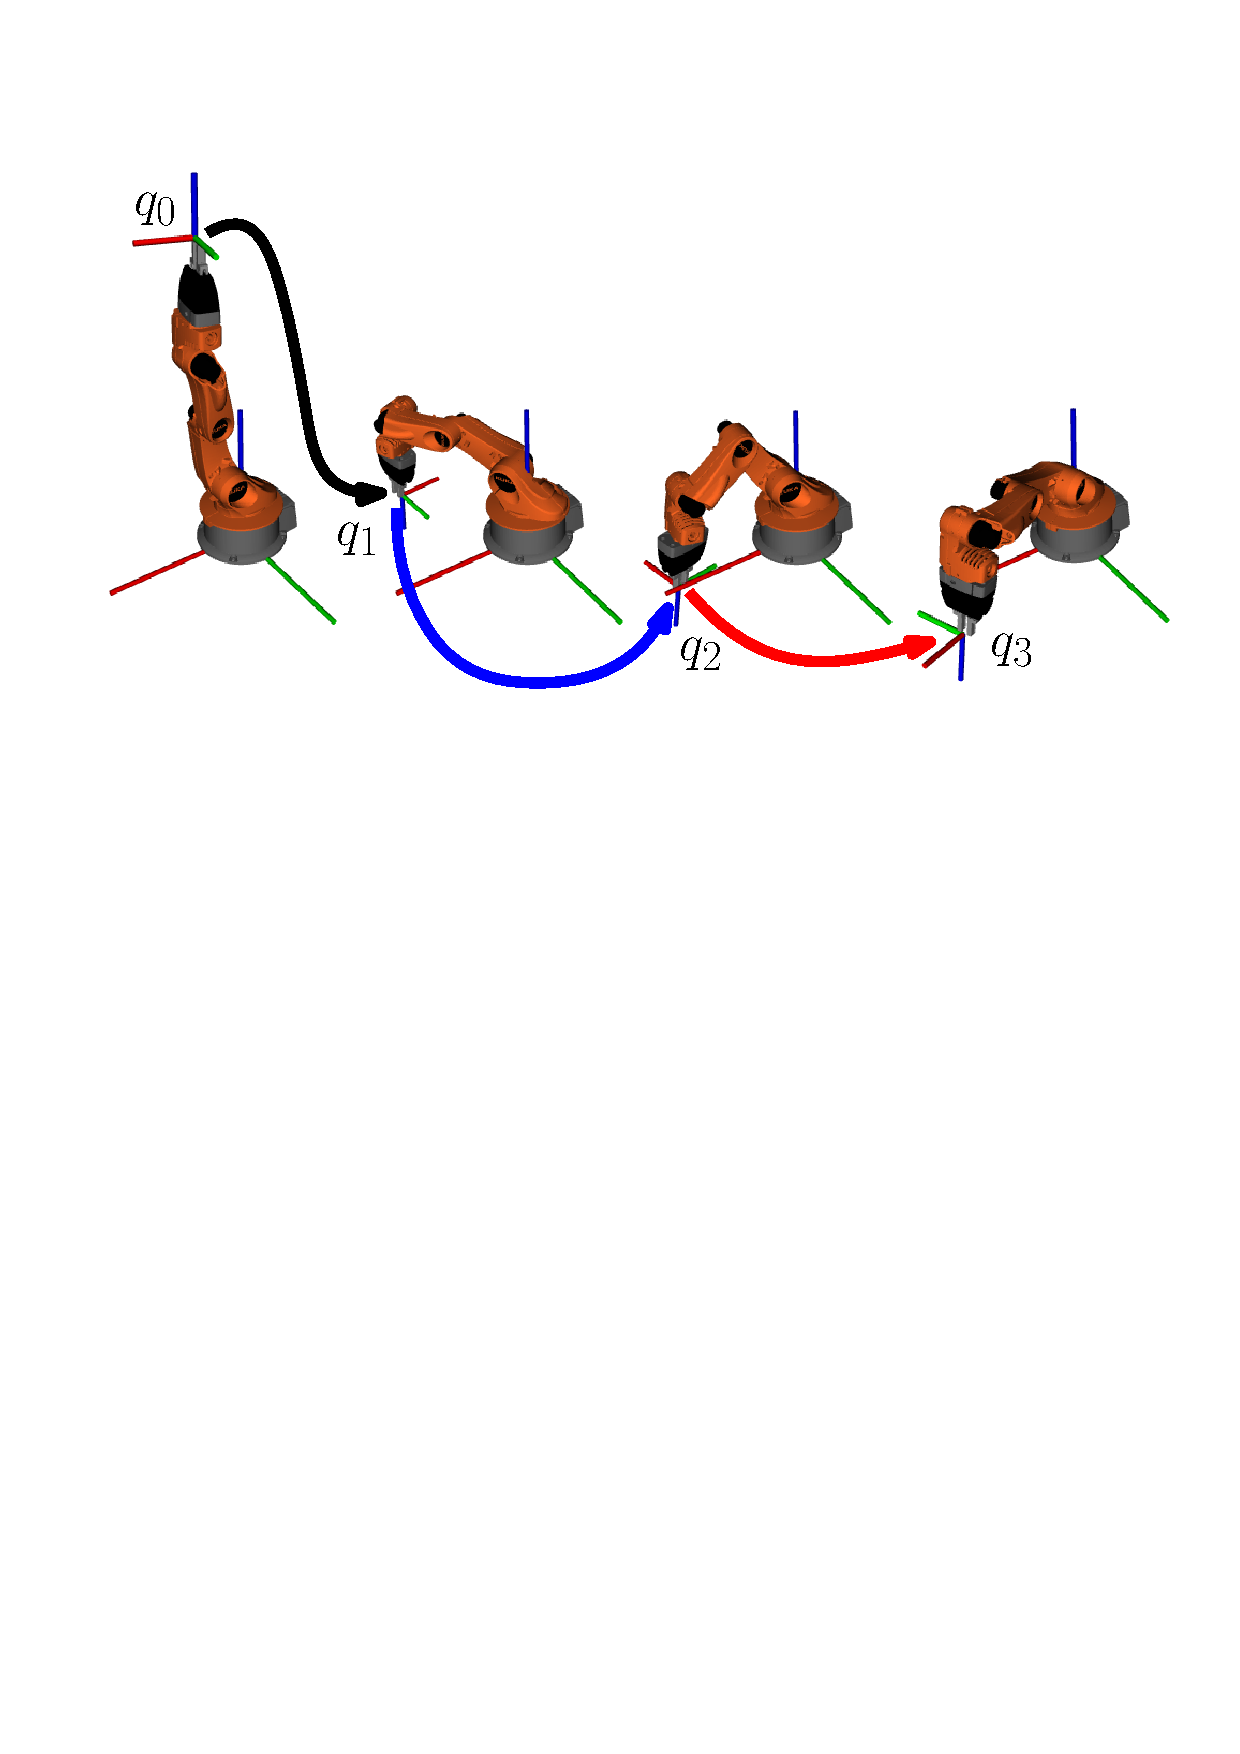
\includegraphics[width=1\textwidth]{modeling/poses.pdf}}
	\caption{Последовательность принятия положений заданных в~\ref{poses_q}}
	\vspace{0.5cm}
	\label{img:poses}
\end{figure}
\begin{gather}\label{poses_q}
	q_0 = 
	\begin{bmatrix}
	2.95 \\ 1.35 \\-2.59 \\1.58\\ 0
	\end{bmatrix}\!\!,\quad
	q_1 =
	\begin{bmatrix}
		 4.06 \\ 2.34\\ -2.2\\ 3.32\\ 1.01
	\end{bmatrix}\!\!,\quad
	q_2 = 
	\begin{bmatrix}
	3.07 \\1.75\\ -0.93 \\2.54\\ 1.73
	\end{bmatrix}\!\!,\quad
	q_3 = 
	\begin{bmatrix}
	2.57\\ 2.33\\ -2.35\\ 3.36\\ 2.97
	\end{bmatrix}\!\!.
\end{gather}

На рисунках~\ref{img:segments_traj} и~\ref{img:polyn_traj} показаны графики переходных процессов для переходов из точки в точку при планировании траектории сегментами и использовании полинома пятой степени соответственно.

\begin{figure}[h!]
	\centering{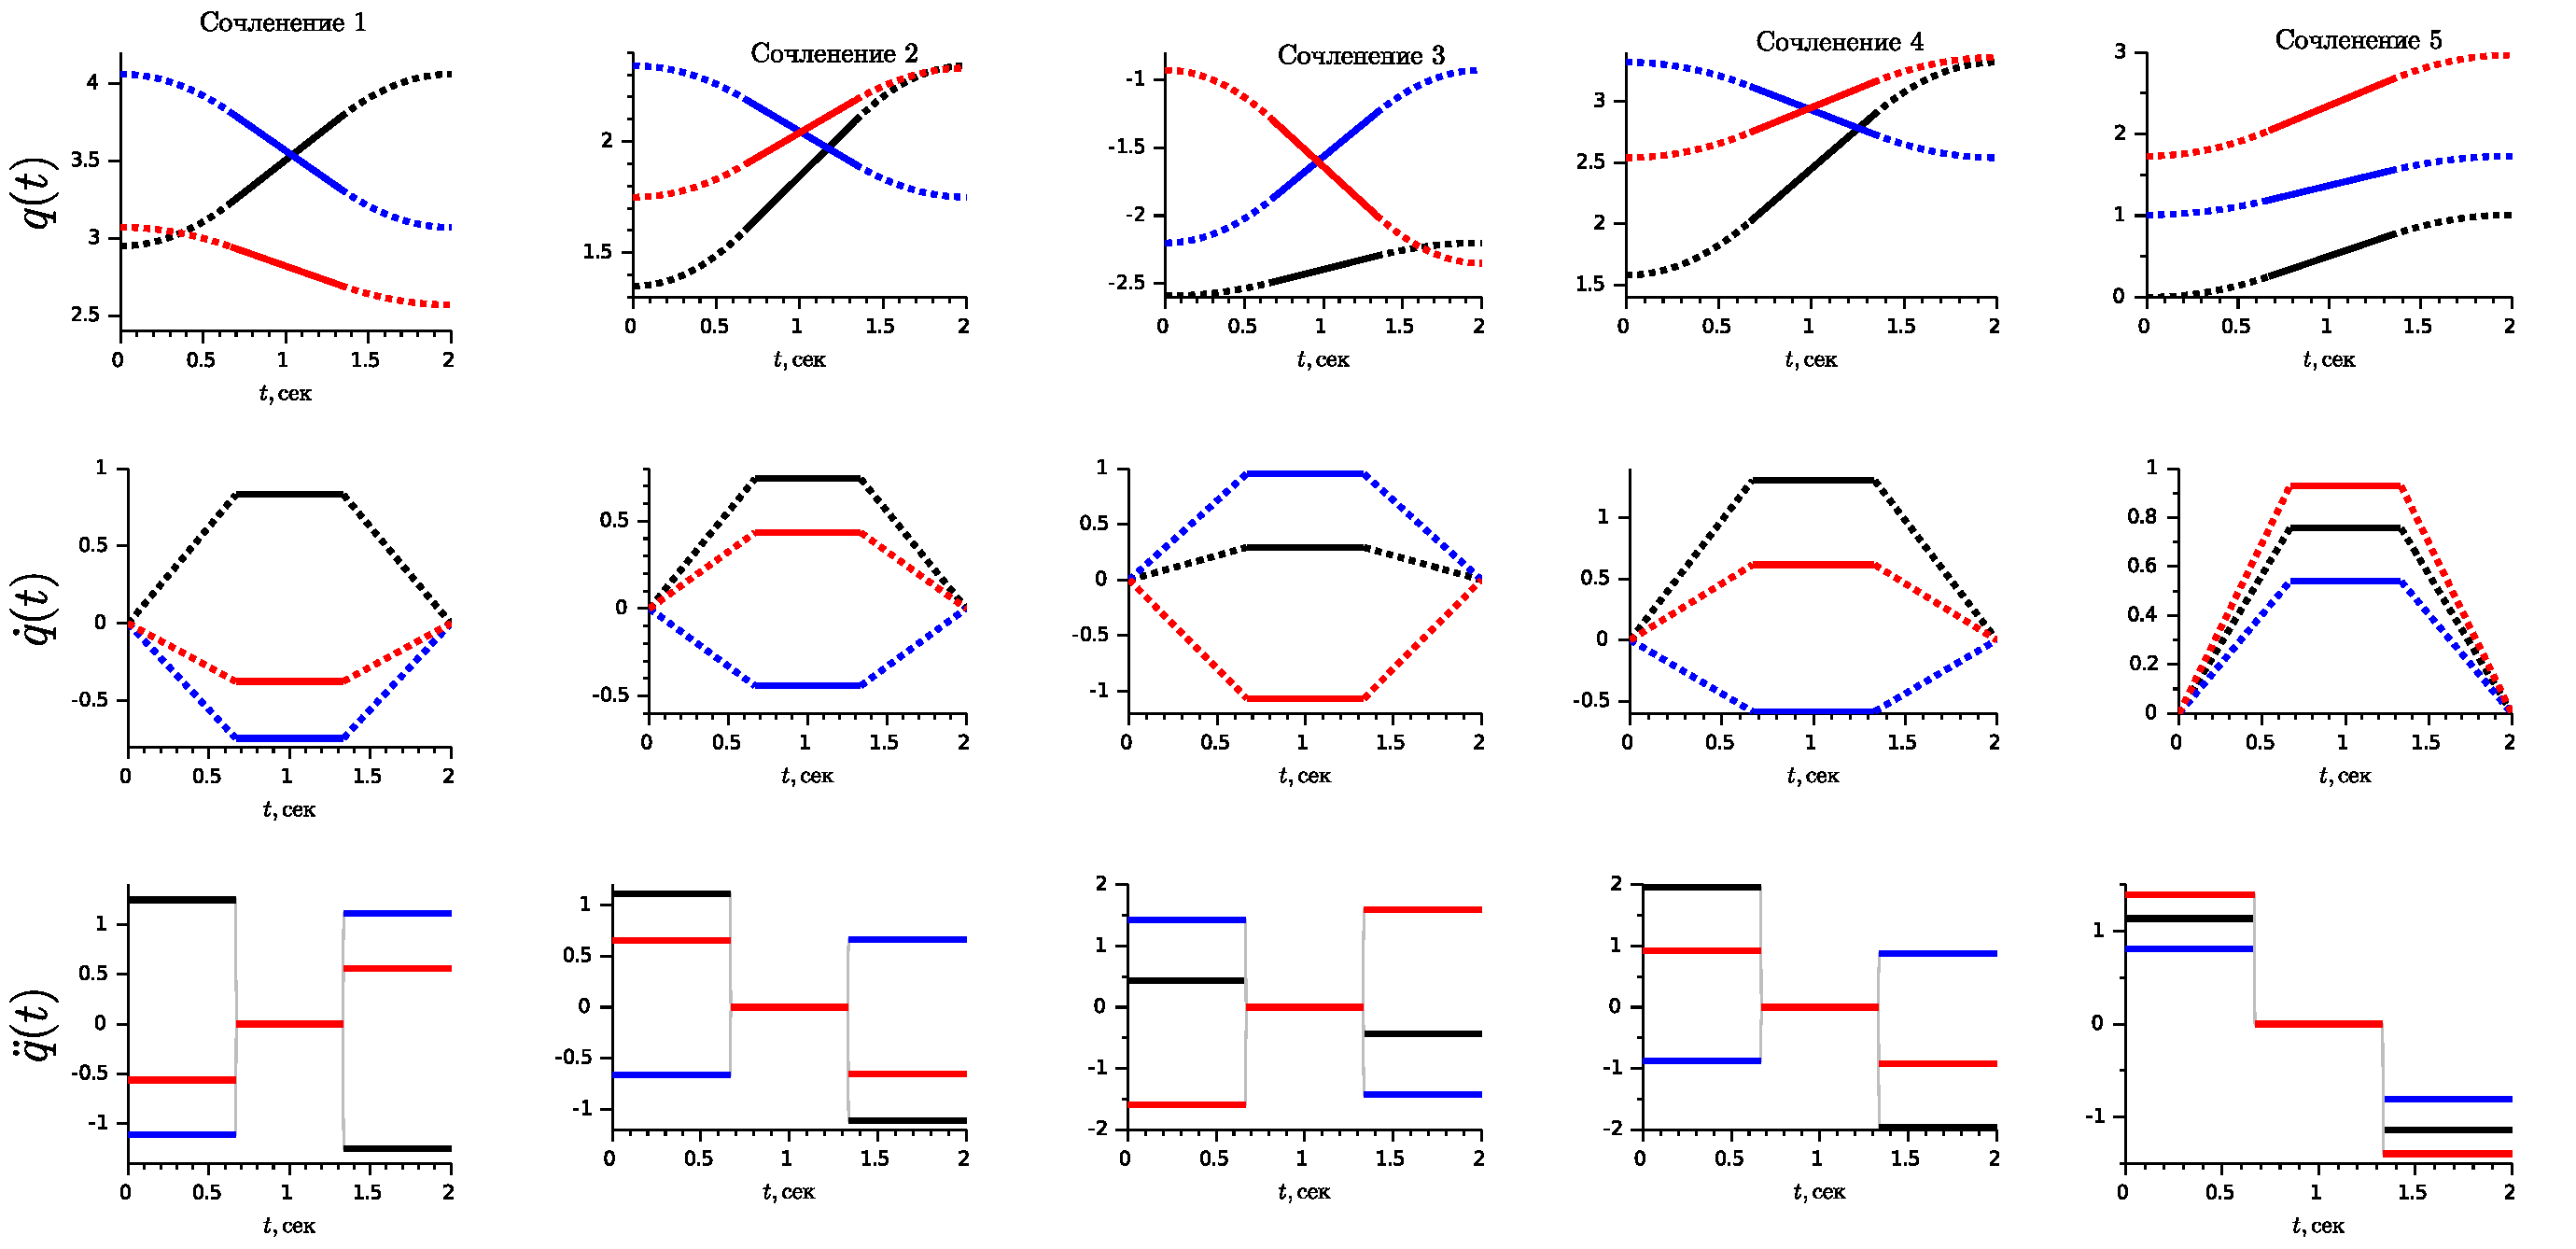
\includegraphics[width=1\textwidth]{modeling/seg_traj.pdf}
		\small черный: для перехода $ q_0 \to q_1 $, \textcolor{blue}{синий: для перехода $ q_1 \to q_2 $}, \textcolor{red}{красный: для перехода $ q_2 \to q_3 $}}
	\vspace{0.2cm}
	\caption{Траектория с трапецеидальным профилем скорости}
	\label{img:segments_traj}
\end{figure}

\begin{figure}[h!]
	\centering{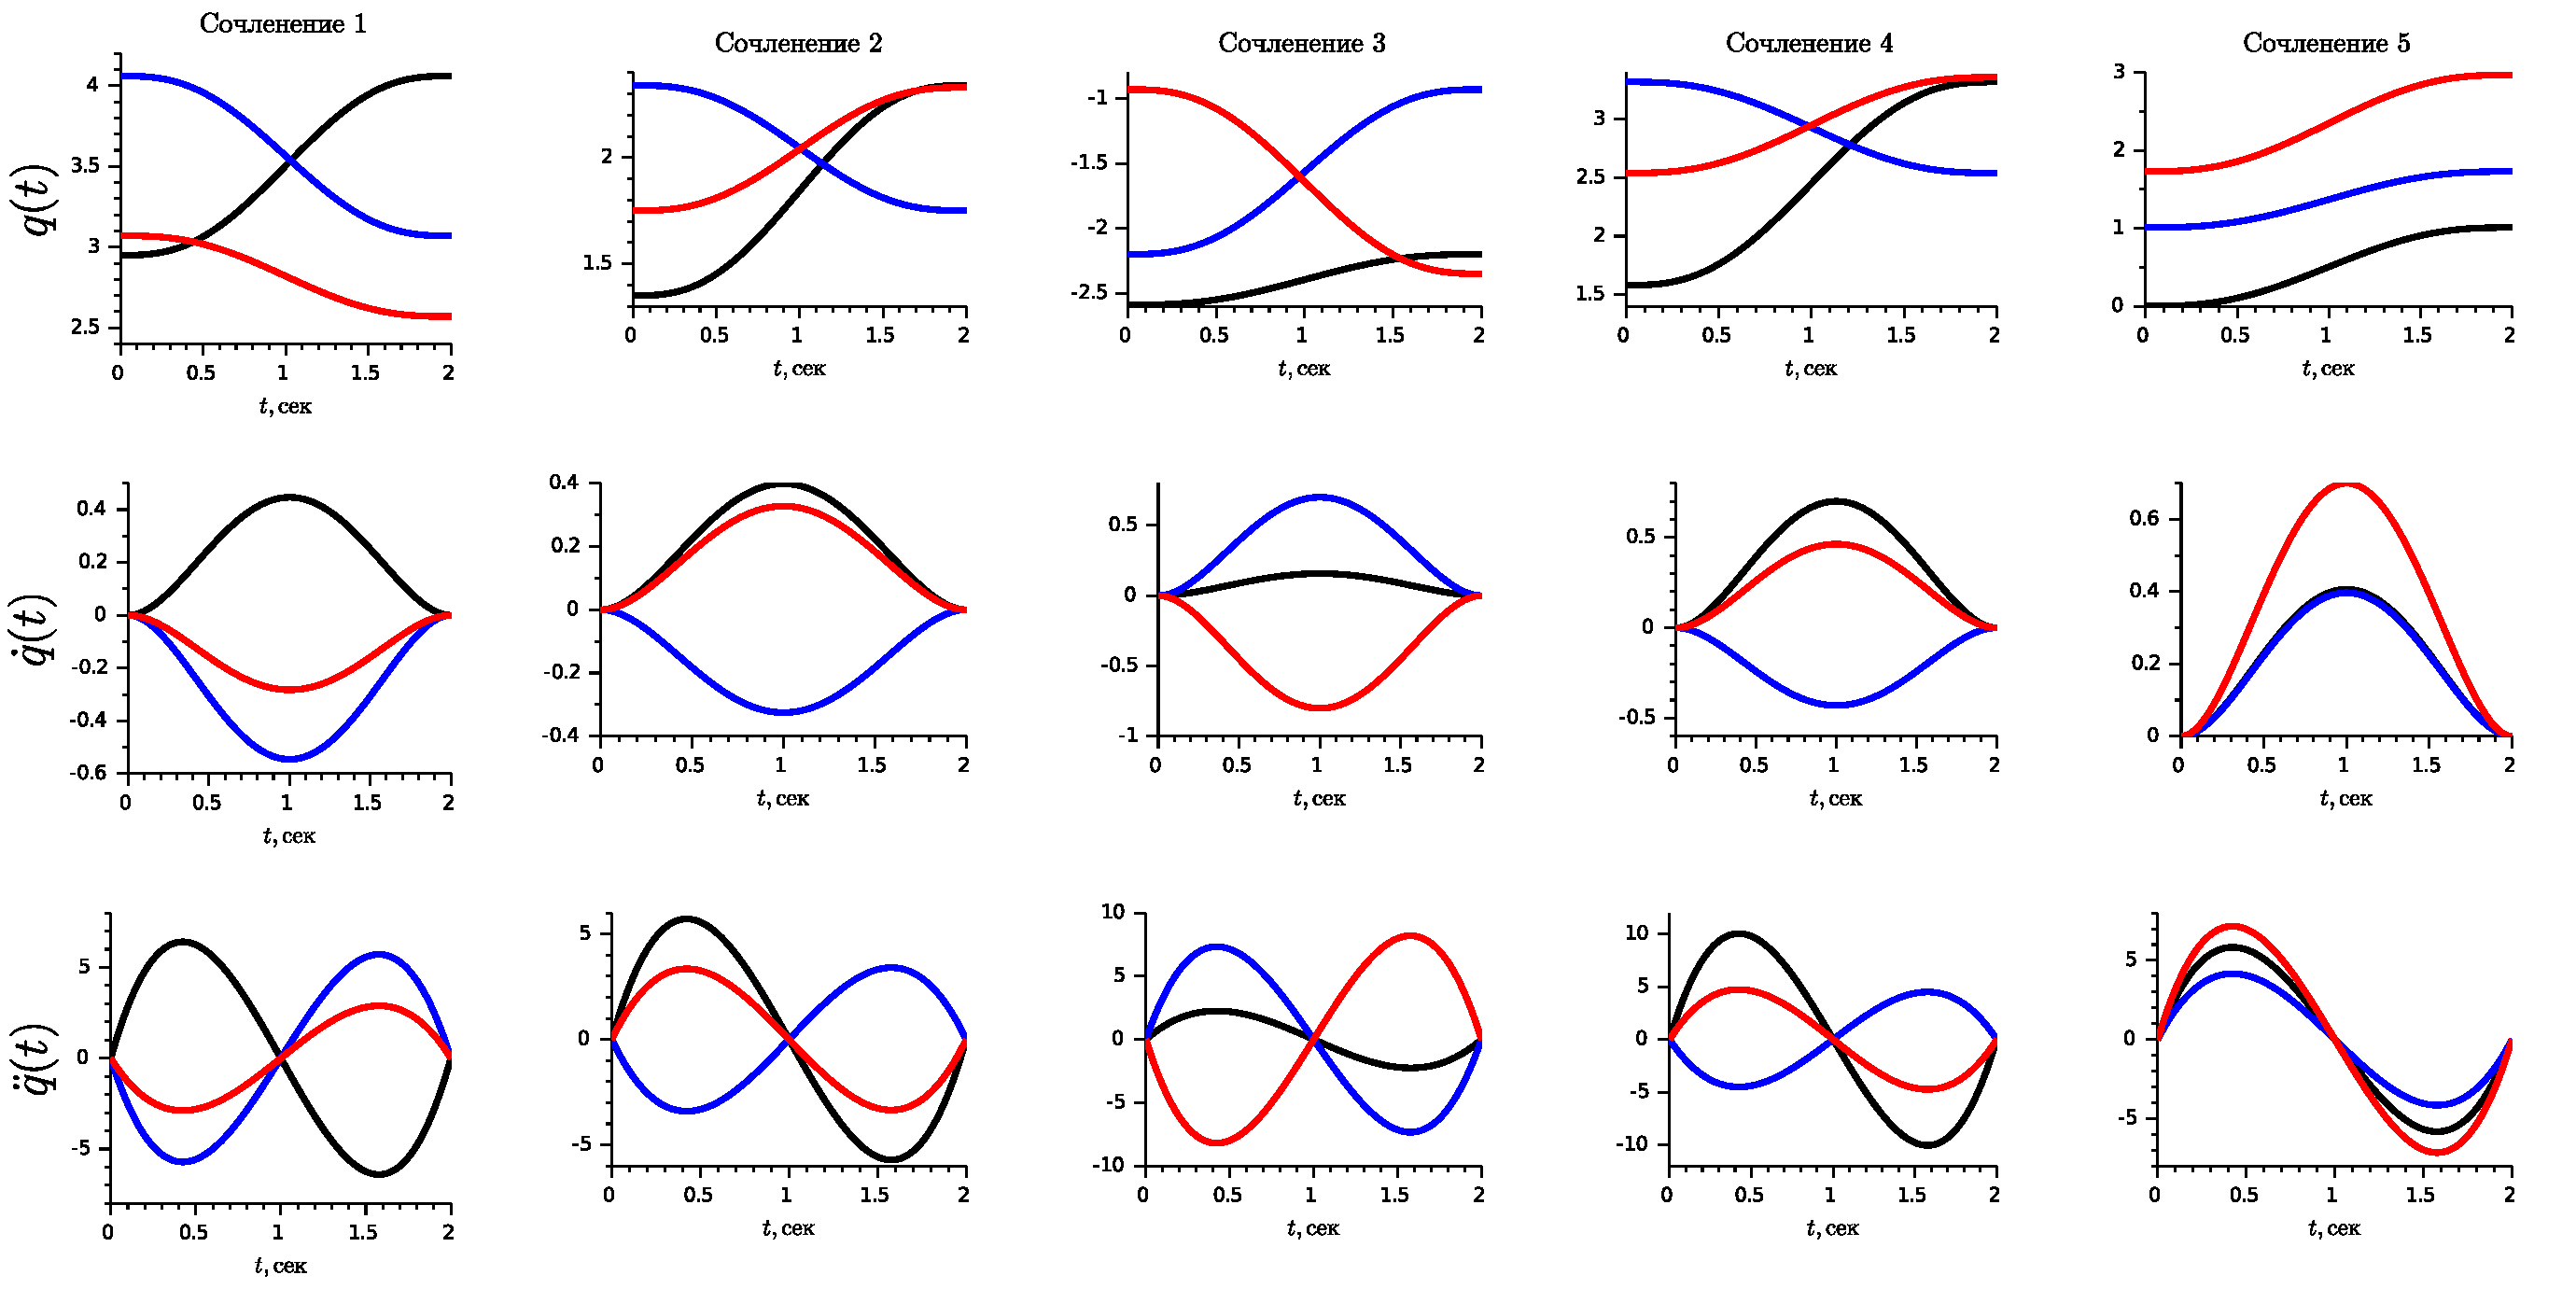
\includegraphics[width=1\textwidth]{modeling/poly_traj.pdf}
		\small черный: для перехода $ q_0 \to q_1 $, \textcolor{blue}{синий: для перехода $ q_1 \to q_2 $}, \textcolor{red}{красный: для перехода $ q_2 \to q_3 $}}
	\vspace{0.2cm}
	\caption{Траектория при полиномиальной интерполяции}
	\label{img:polyn_traj}
\end{figure}

\begin{figure}[h!]
	\centering{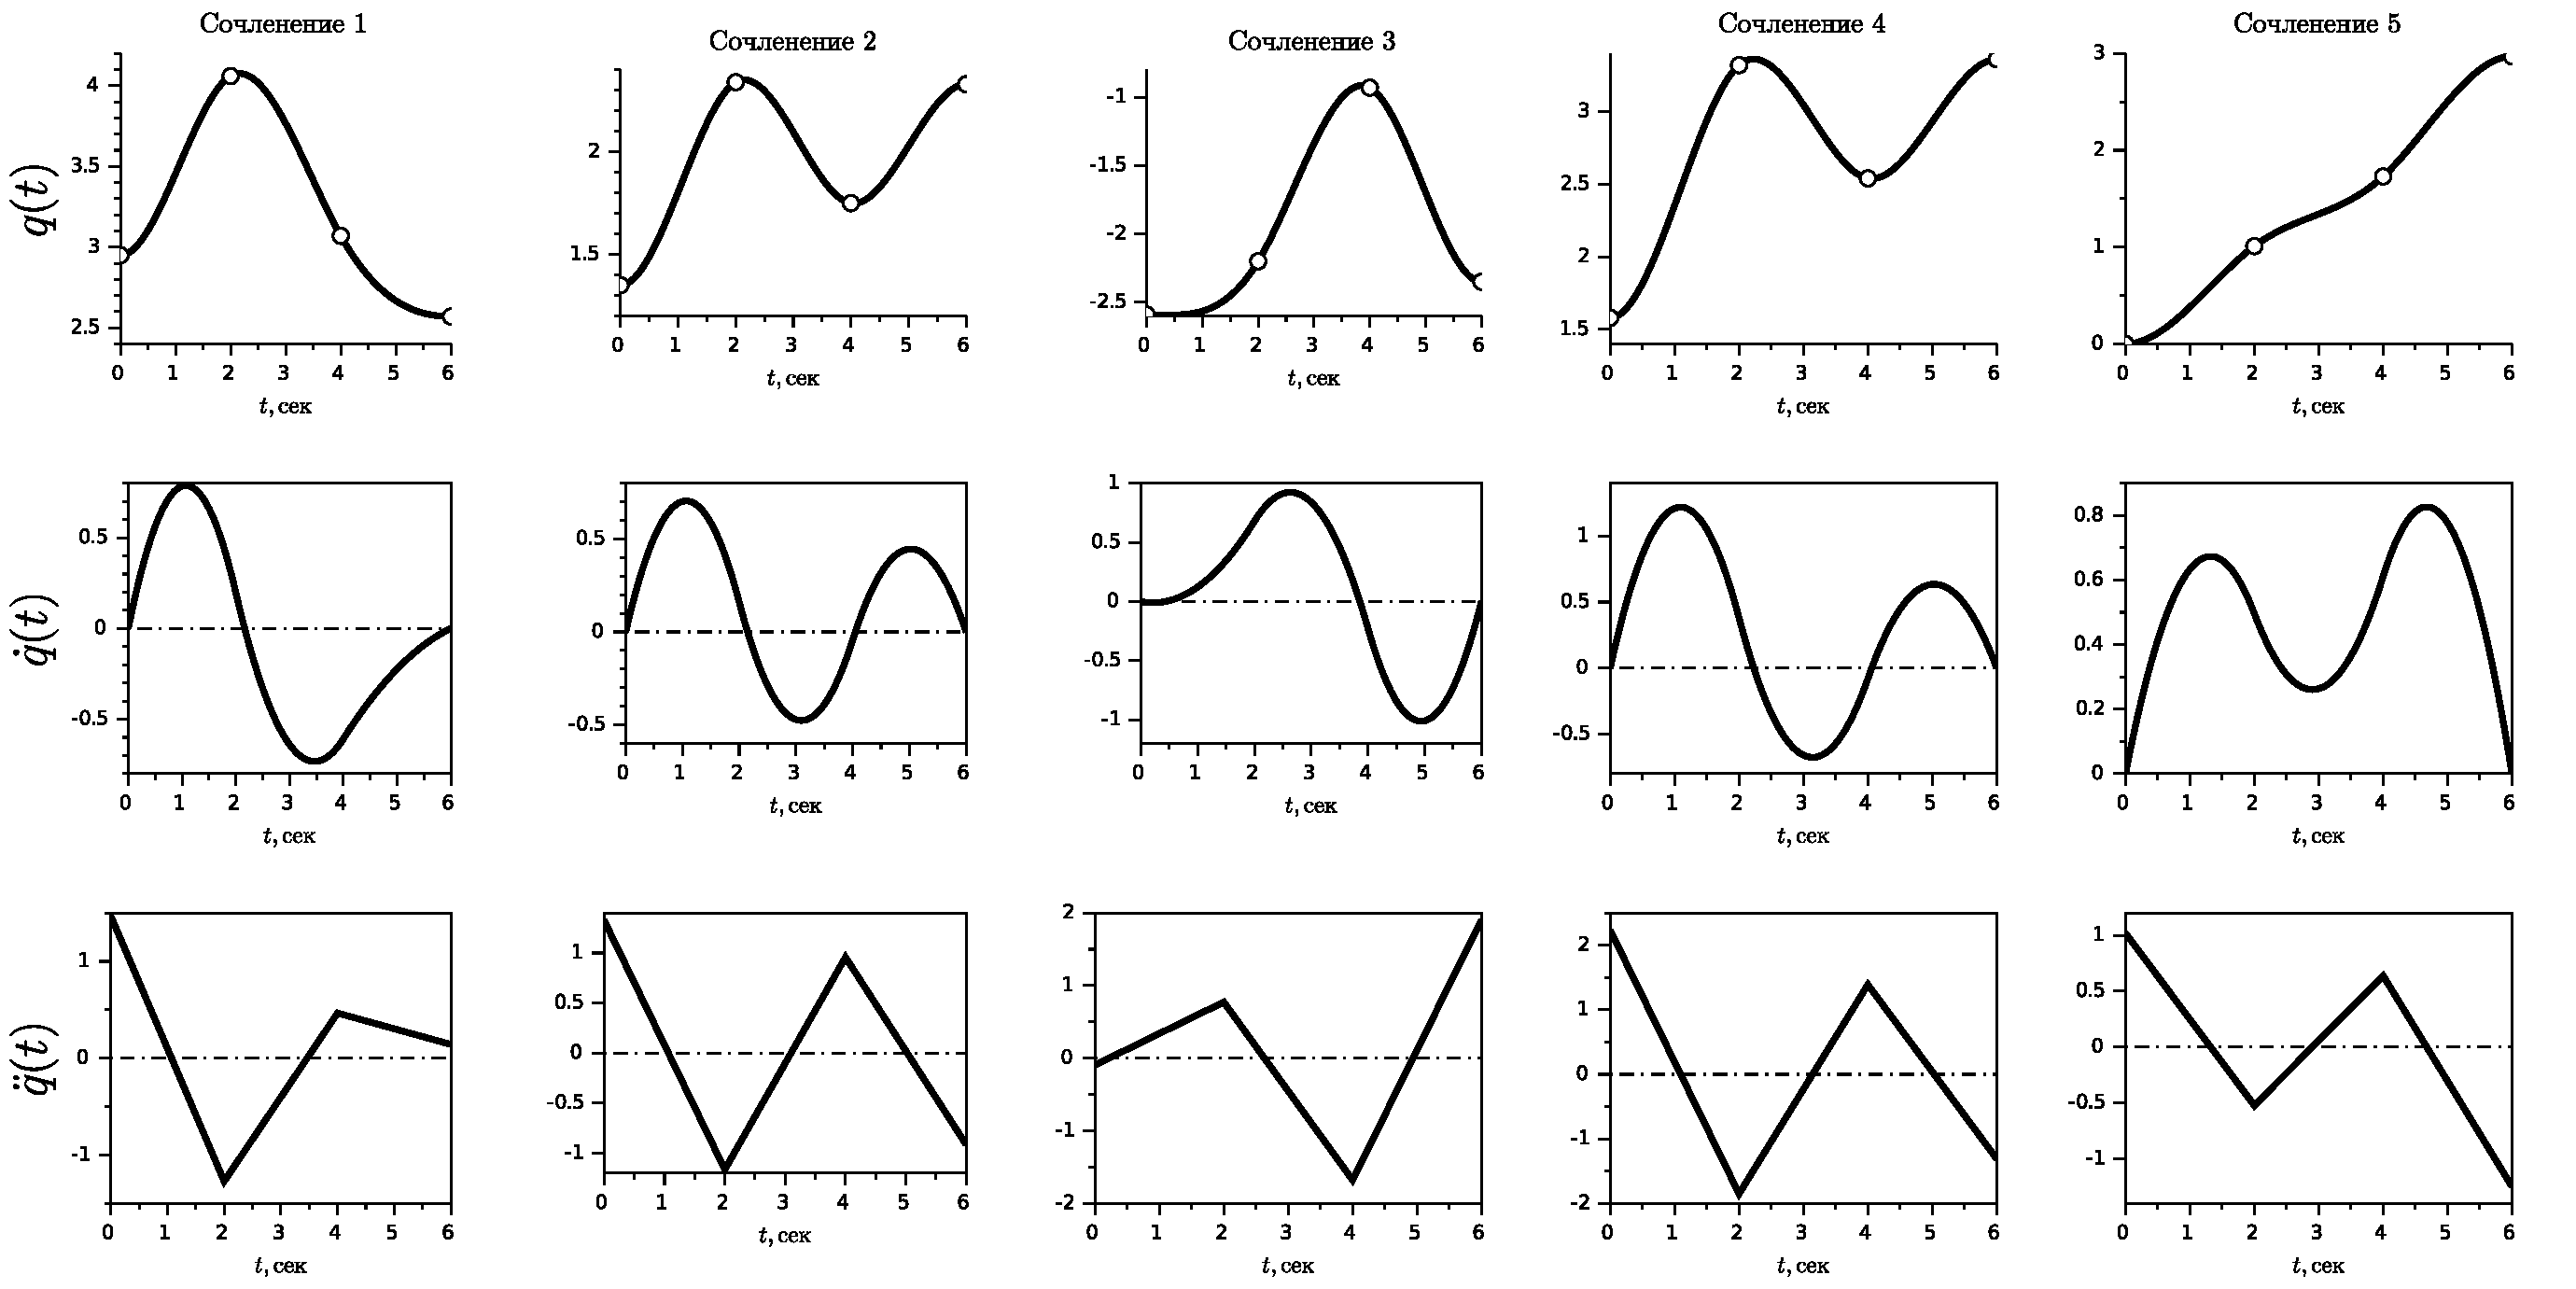
\includegraphics[width=1\textwidth]{modeling/spline_traj.pdf}
		\small узлы на верхних графиках представляют из себя точки $ q_0(0), q_1(2), q_2(4), q_3(6) $}
	\vspace{0.2cm}
	\caption{Непрерывная траектория через набор точек}
	\label{img:spline_traj}
\end{figure}

Траектория (дуга) в операционном пространстве и соответствующие ей траектории каждого из сочленений в конфигурационном пространстве представлены на рисунке~\ref{img:cartesian}.

\begin{figure}[h!]
	\centering{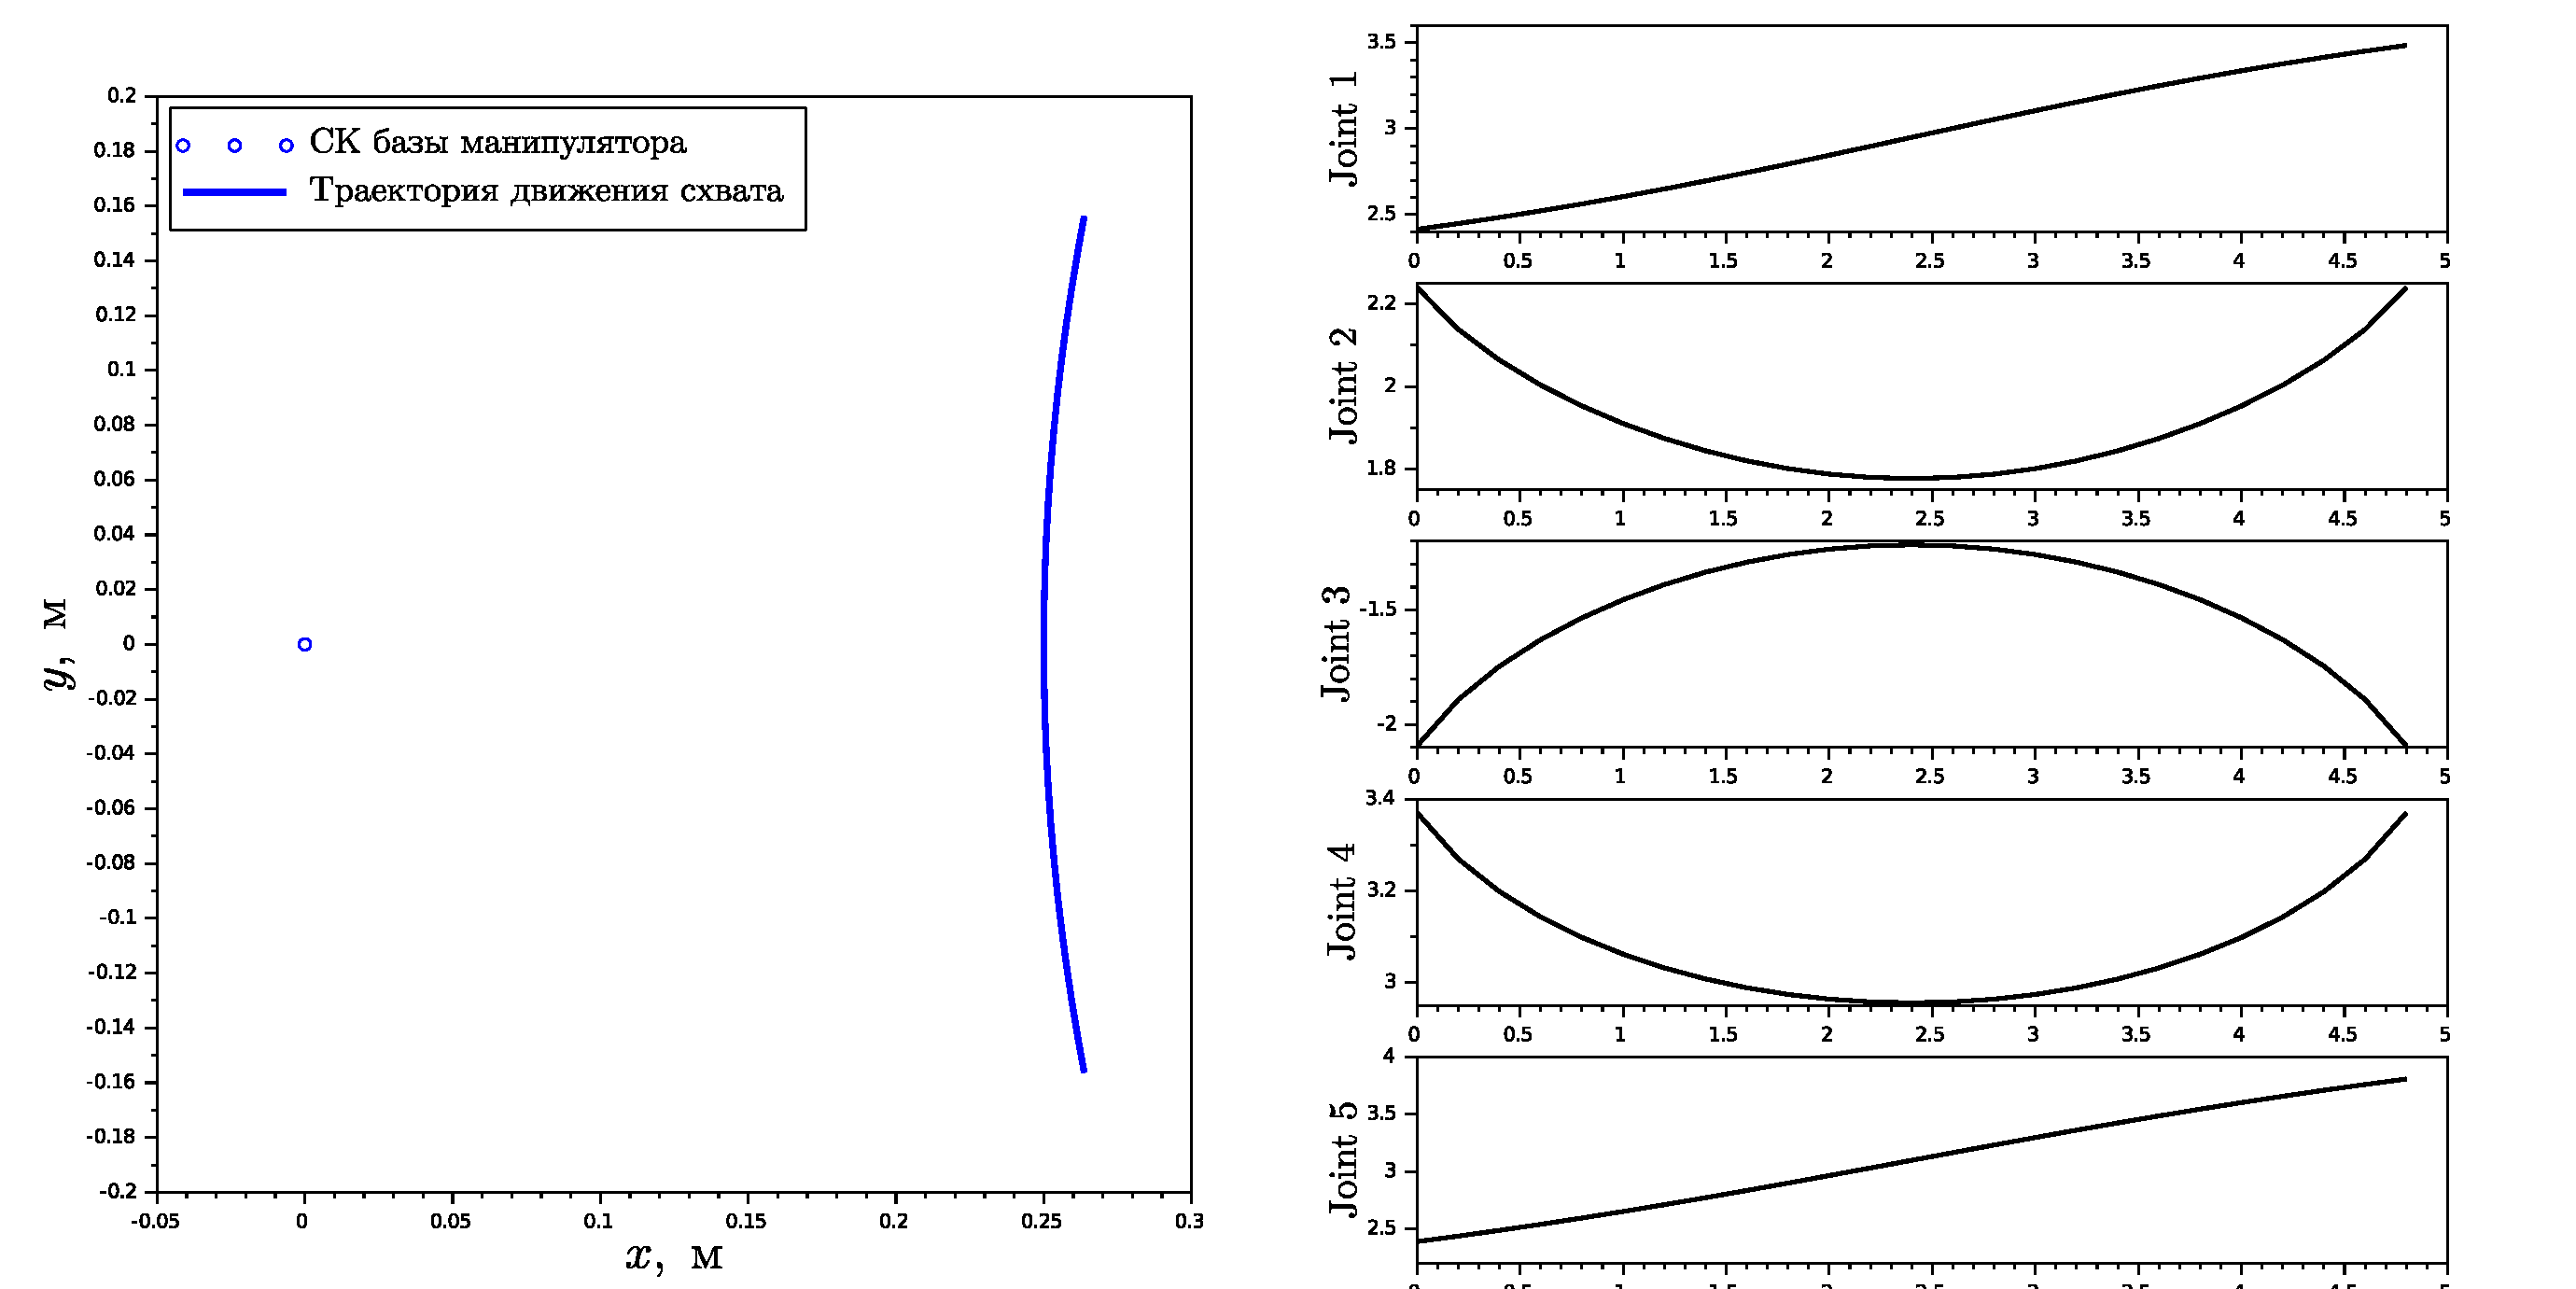
\includegraphics[width=1\textwidth]{modeling/cartesian.pdf}}
	\vspace{0.2cm}
	\caption{Траектория движения схвата манипулятора и соответствующие ей траектории сочленений в конфигурационном пространстве}
	\label{img:cartesian}
\end{figure}

\begin{figure}[h!]
	\centering{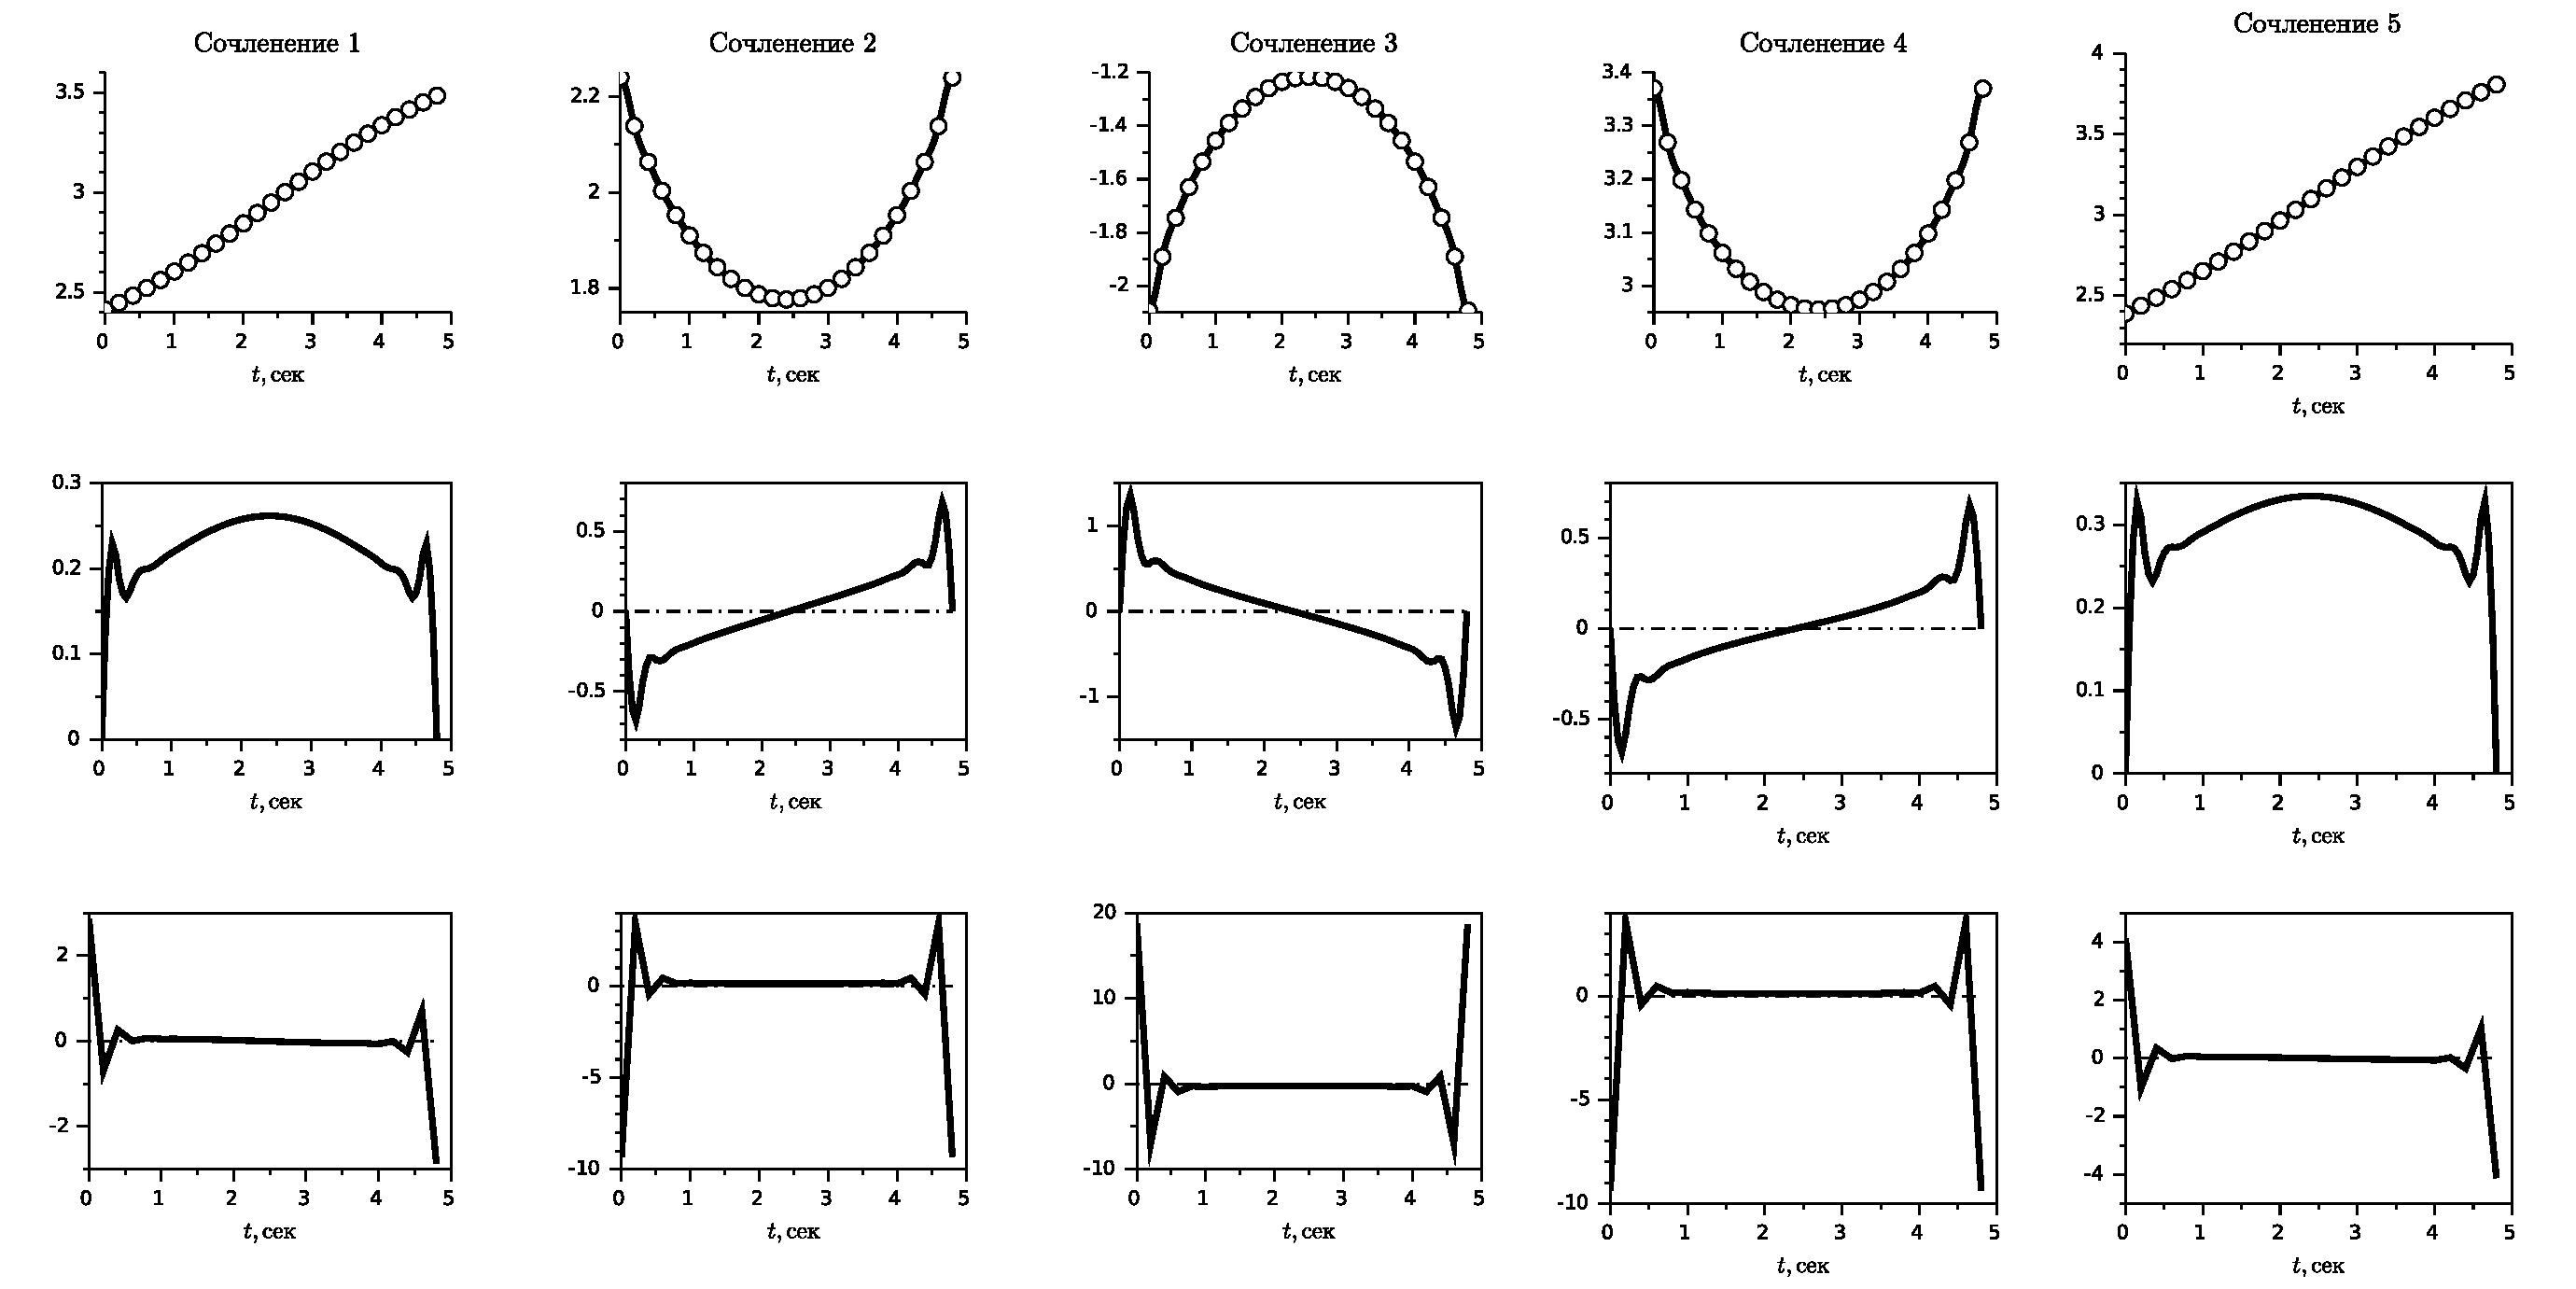
\includegraphics[width=1\textwidth]{modeling/js_cartesian.pdf}}
	\vspace{0.2cm}
	\caption{Интерполяция траекторий кубическими сплайнами}
	\label{img:js_cartesian}
\end{figure}

\clearpage

\subsection{Моделирование системы управления манипулятором}

\begin{figure}[h!]
	\centering{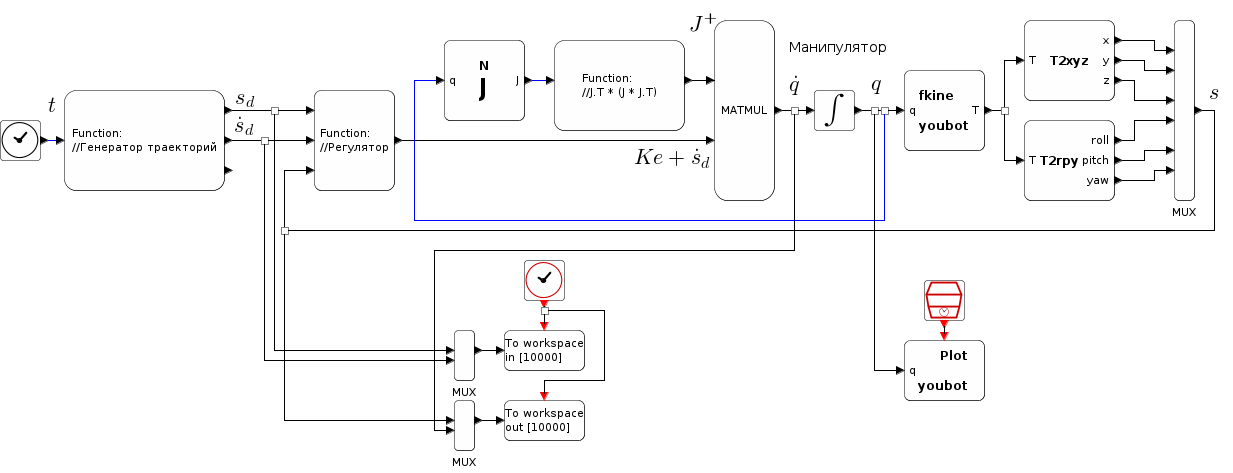
\includegraphics[width=0.95\textwidth]{modeling/control_system.png}}
	\caption{Модель системы управления манипуляторов в Scilab}
	\label{img:control_system}
\end{figure}

\begin{figure}[h!]
	\begin{minipage}[h]{0.5\linewidth}
		\centering{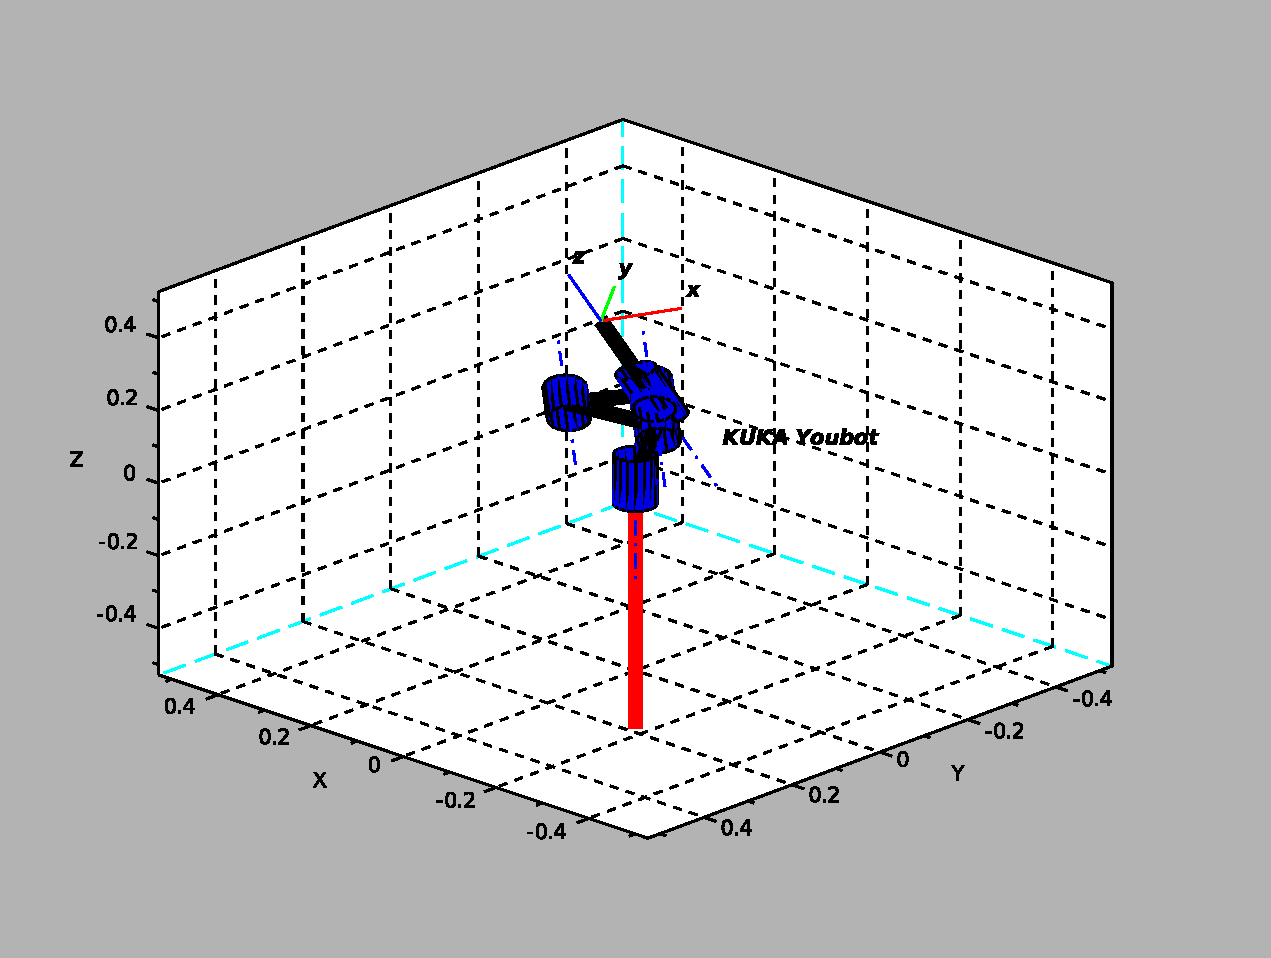
\includegraphics[width=1\linewidth]{modeling/model1.pdf} \\ а)}
	\end{minipage}
	\hfill
	\begin{minipage}[h]{0.5\linewidth}
		\centering{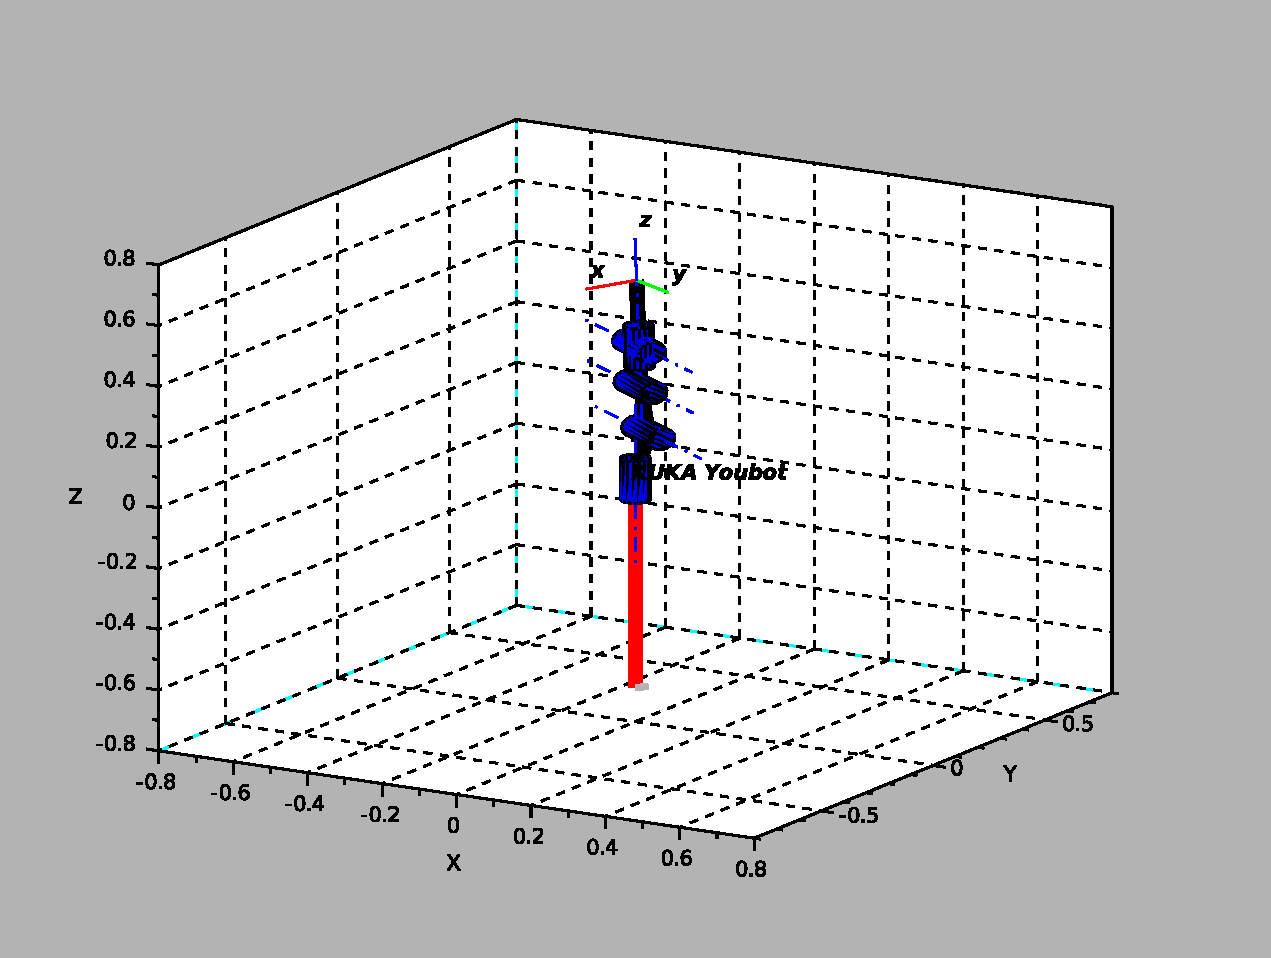
\includegraphics[width=1\linewidth]{modeling/model2.pdf} \\ б)}
	\end{minipage}
	\caption{a) Манипулятор KUKA YouBot в "домашней" конфигурации; б) В свече}
	\label{img:model}
\end{figure}

\subsection{Результаты работы системы технического зрения}

Путь получения координат и ориентации объекта покажем на нижеследующей последовательности рисунков. На рисунке~\ref{img:raw_cloud} изображено облако точек, полученное с камеры Intel RealSense SR300. После фильтрации этого облака, получается облако с пониженным качеством и показывается на рисунке~\ref{img:downsampled_cloud}. Далее, на рисунке~\ref{img:downsampled_cloud}б, изображена плоскость~--- результат работы алгоритма сегментации. Следующий рисунок~\ref{img:hull}а содержит результат нахождения выпуклой оболочки вокруг плоскости. И, облако точек целевого объекта, показоно на рисунке~\ref{img:hull}б. Рисунок~\ref{img:frame} включает плоскость, объект и СК прикрепленную к объекту.

\begin{figure}[h!]
	\begin{minipage}[h]{0.5\linewidth}
		\centering{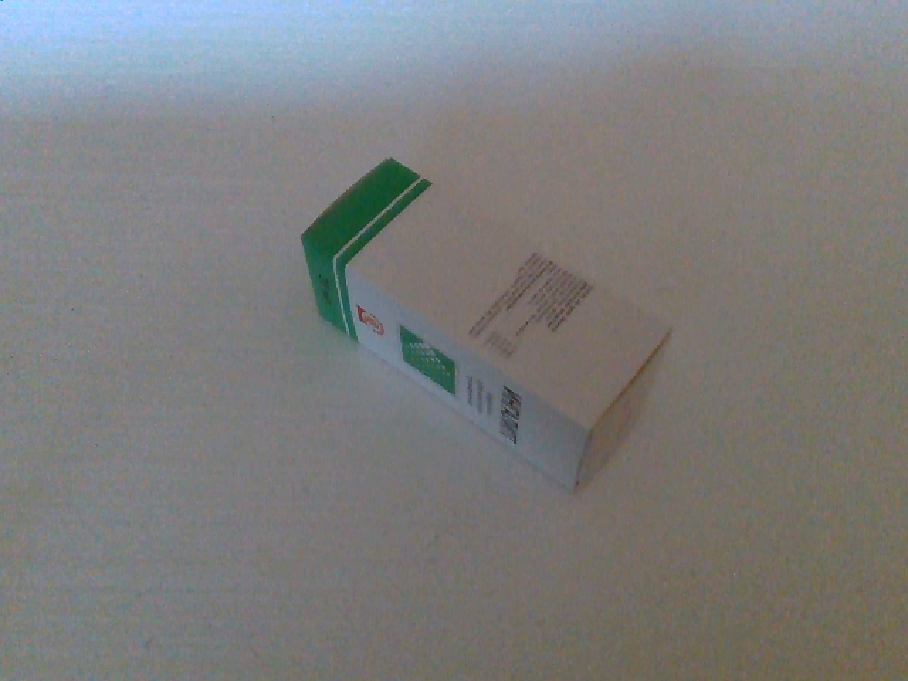
\includegraphics[width=0.7\linewidth]{modeling/cv_image.png} \\ а)}
	\end{minipage}
	\hfill
	\begin{minipage}[h]{0.5\linewidth}
		\centering{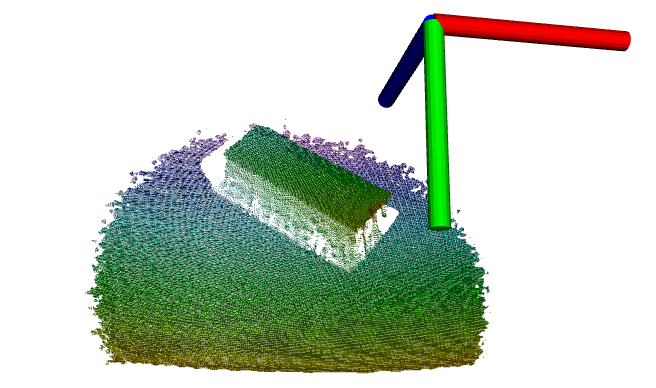
\includegraphics[width=1\linewidth]{modeling/cv_raw_cloud.png} \\ б)}
	\end{minipage}
	\caption{a) Цветное изображение целевого объекта; б) Необработанное облако точек}
	\label{img:raw_cloud}
\end{figure}

\begin{figure}[h!]
	\begin{minipage}[h]{0.5\linewidth}
		\centering{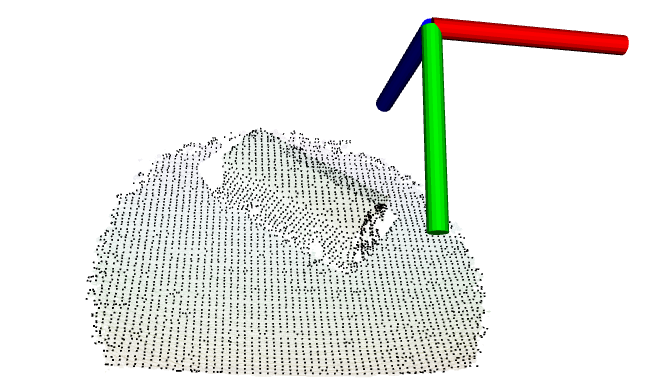
\includegraphics[width=1\linewidth]{modeling/_cv_raw_ds.png} \\ а)}
	\end{minipage}
	\hfill
	\begin{minipage}[h]{0.5\linewidth}
		\centering{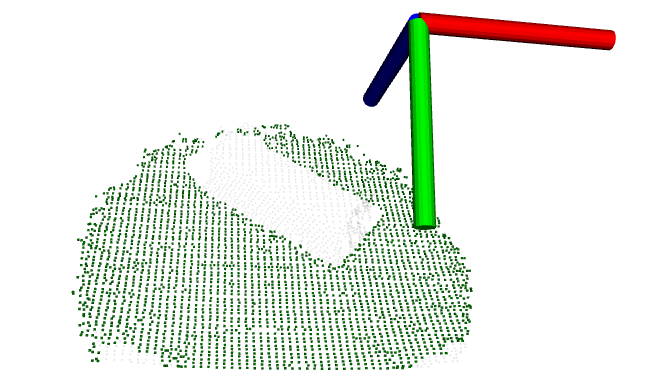
\includegraphics[width=1\linewidth]{modeling/_cv_ds2plane.png} \\ б)}
	\end{minipage}
	\caption{а) Облако точек пропущенное через фильтр VoxelGrid; б) Часть облака точек принадлежащая плоскости в кадре самой большой площади}
	\label{img:downsampled_cloud}
\end{figure}

\begin{figure}[h!]
	\begin{minipage}[h]{0.5\linewidth}
		\centering{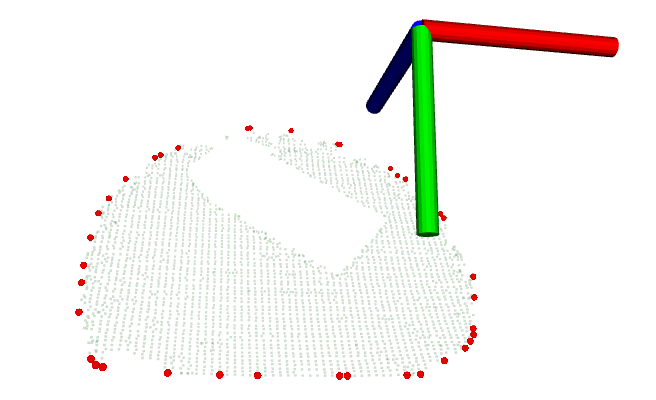
\includegraphics[width=1\linewidth]{modeling/_cv_plane2hull.png} \\ а)}
	\end{minipage}
	\hfill
	\begin{minipage}[h]{0.5\linewidth}
		\centering{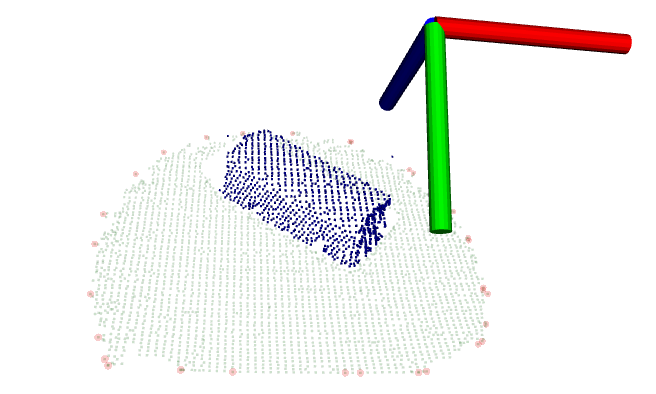
\includegraphics[width=1\linewidth]{modeling/_cv_2object.png} \\ б)}
	\end{minipage}
	\caption{а) Точки принадлежащие выпуклой оболочке, вокруг плоскости; б) Кластер облака точек включающих только целевой объект}
	\label{img:hull}
\end{figure}

\begin{figure}[h!]
	\centering{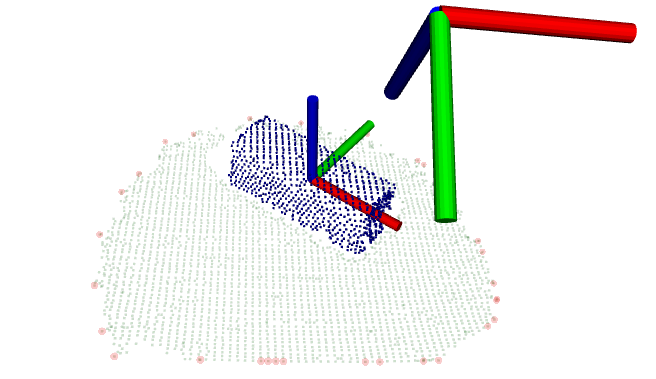
\includegraphics[width=1\textwidth]{modeling/cv_frame.png}}
	\vspace{0.2cm}
	\caption{Прикрепленная к объекту СК}
	\label{img:frame}
\end{figure}

\clearpage
\newpage